\section{JavaScript Semantics Specialization with Syntactic Views}\label{sec:formal}

We first define $\ires$ as a specification language to describe JavaScript
semantics.

\subsection{$\ires$: Intermediate Representations for ECMAScript}

We first introduce $\ires$, an \textbf{I}ntermediate \textbf{R}epresentations
for \textbf{E}CMA\textbf{S}cript, as a specification language for JavaScript to
describe JavaScript semantics. We define its abstract syntax, states, and
concrete semantics in the remainder of this section.

\subsubsection{Abstract Syntax}

\[
  \begin{array}{lr@{~}c@{~}c@{~}c@{~}l}
    \text{Programs} & \progset &\ni& \prog &=& (\istset, \getfunc, \getinst,
    \getnext)\\

    \text{Functions} & \funcset &\ni& \func &::=&
    \kwdef \; \kwrl \varx^* \kwrr \; \lab\\

    \text{Variables} & \varset &\ni& \varx\\

    \text{Instructions} & \instset &\ni& \inst &::=&
    \refer = \expr \mid
    \varx = \kwcl \kwcr \mid
    \varx = \expr \kwrl \expr^* \kwrr \mid \\&&&&&
    \kwif \; \expr \; \lab \; \lab \mid
    \kwret \; \expr\\

    \text{Labels} & \labset &\ni& \lab\\

    \text{Expressions} & \exprset &\ni& \expr &::=&
    \pval \mid
    \op \kwrl \expr^* \kwrr \mid
    \refer\\

    \text{References} & \referset &\ni& \refer &::=&
    \varx \mid \expr \kwsl \expr \kwsr\\
  \end{array}
\]

An $\ires$ program $\prog = (\istset, \getfunc, \getinst, \getnext) \in \progset $
consists of initial states and three mappings; $\getfunc: \labset \rightarrow
\funcset$ and $\getinst: \labset \rightarrow \instset$ map labels to their
functions and instructions, respectively, and $\getnext: \labset \rightarrow
\labset$ maps labels to their next labels, where a label $\lab \in \labset$
denotes a program point.  A function $\func \in \funcset$ is defined with its
parameters and body label.  For presentation brevity, we assume that no global
or captured variables exist in this paper.  An instruction $\inst \in \instset$
is an assignment $\refer = \expr$, an object allocation $\varx = \kwcl \kwcr$, a
function call $\varx = \expr \kwrl \expr^* \kwrr$, a branch $\kwif \; \expr \;
\lab \; \lab$, or a return instruction $\kwret \; \expr$.  An invocation of an
abstract algorithm in ECMAScript is compiled to a function call instruction with
a new temporary variable.  We represent loops using branch instructions with
cyclic pointing of labels in $\getnext$.  An expression is a primitive value
$\pval$, an operation $\op \kwrl \expr^* \kwrr$, or a reference $\refer$.  A
reference is a variable $\varx$ or an object field $\expr \kwsl \expr \kwsr$.
We write $\expr.\varf$ to briefly represent $\expr \kwsl \code{"f"} \kwsr$.


\subsubsection{States}

\[
  \begin{array}{lr@{~}c@{~}l@{~}c@{~}l}
    \text{States} & \st &\in& \stset &=&
    \labset \times \ctxtset^* \times \heapset \times \envset\\

    \text{Calling Contexts} & \ctxt &\in& \ctxtset &=&
    \labset \times \envset \times \varset\\

    \text{Heaps} & \heap &\in& \heapset &=&
    \addrset \finmap \objset\\

    \text{Objects} & \obj &\in& \objset &=&
    \strset \finmap \valset\\

    \text{Environments} & \env &\in& \envset &=&
    \varset \finmap \valset\\

    \text{Values} & \val &\in& \valset &=&
    \pvalset \uplus \addrset \uplus \treeset \uplus \funcset\\

    \text{Primitive Values} & \pval &\in& \pvalset &=&
    \boolset \uplus \intset \uplus \strset \uplus \cdots\\

    \text{JavaScript ASTs} & \tree &\in& \treeset\\
  \end{array}
\]

States $\stset$ consist of labels $\labset$, calling context stacks
$\ctxtset^*$, heaps $\heapset$, and environments $\envset$.  A calling context
$\ctxt \in \ctxtset$ consists of a label denoting the return point, a caller's
environment, and a return variable.  A heap $\heap \in \heapset$ is a finite
mapping from addresses to objects, and an object $\obj \in \objset$ is a finite
mappings from strings to values.  Each object allocation $\kwcl \kwcr$ creates a
unique address $\addr \in \addrset$ different from existing addresses.  An
environment $\env \in \envset$ is a finite mapping from variables to values. A
value $\val \in \valset$ is a primitive value $\pval \in \pvalset$ (e.g., a
boolean value $\bool \in \boolset$, an integer $k \in \intset$, or a string
$\str \in \strset$), an address $\addr \in \addrset$, a JavaScript AST $\tree
\in \treeset$, or a function $f \in \funcset$.

Since $\ires$ is a specification language for JavaScript, it treats JavaScript
ASTs $\treeset$ as its values. For presentation brevity, we represent a JavaScript
AST as follows:
\[
  \tree ::= \term{\str} \mid \ty_k \langle \tree^* \rangle
\]
A leaf node $\term{\str}$ defined with a string $\str$ denotes a terminal
symbol, and a non-leaf node $\ty_k \langle \tree^* \rangle$ denotes $k$-th
alternative in the syntactic production of nonterminal symbol $\ty$ with its
subtrees $\tree^*$.  The notation $\ty_k.\eval$ denotes an $\ires$ function for
the evaluation of $k$-th alternative in $\ty$, and it takes the AST itself and
its nonterminal subtrees as arguments. If an AST $\tree$ is a subtree of another
AST $\tree'$, we represent it as $\tree \subtree \tree'$.  For example,
Figure~\ref{fig:coalesce-prod} shows a syntactic production for coalesce
expressions.  Consider the following coalesce expression:
\begin{lstlisting}[style=JS]
                    42 ?? true
\end{lstlisting}
Then, the following AST is produced as its parsing result:
\begin{figure}[H]
  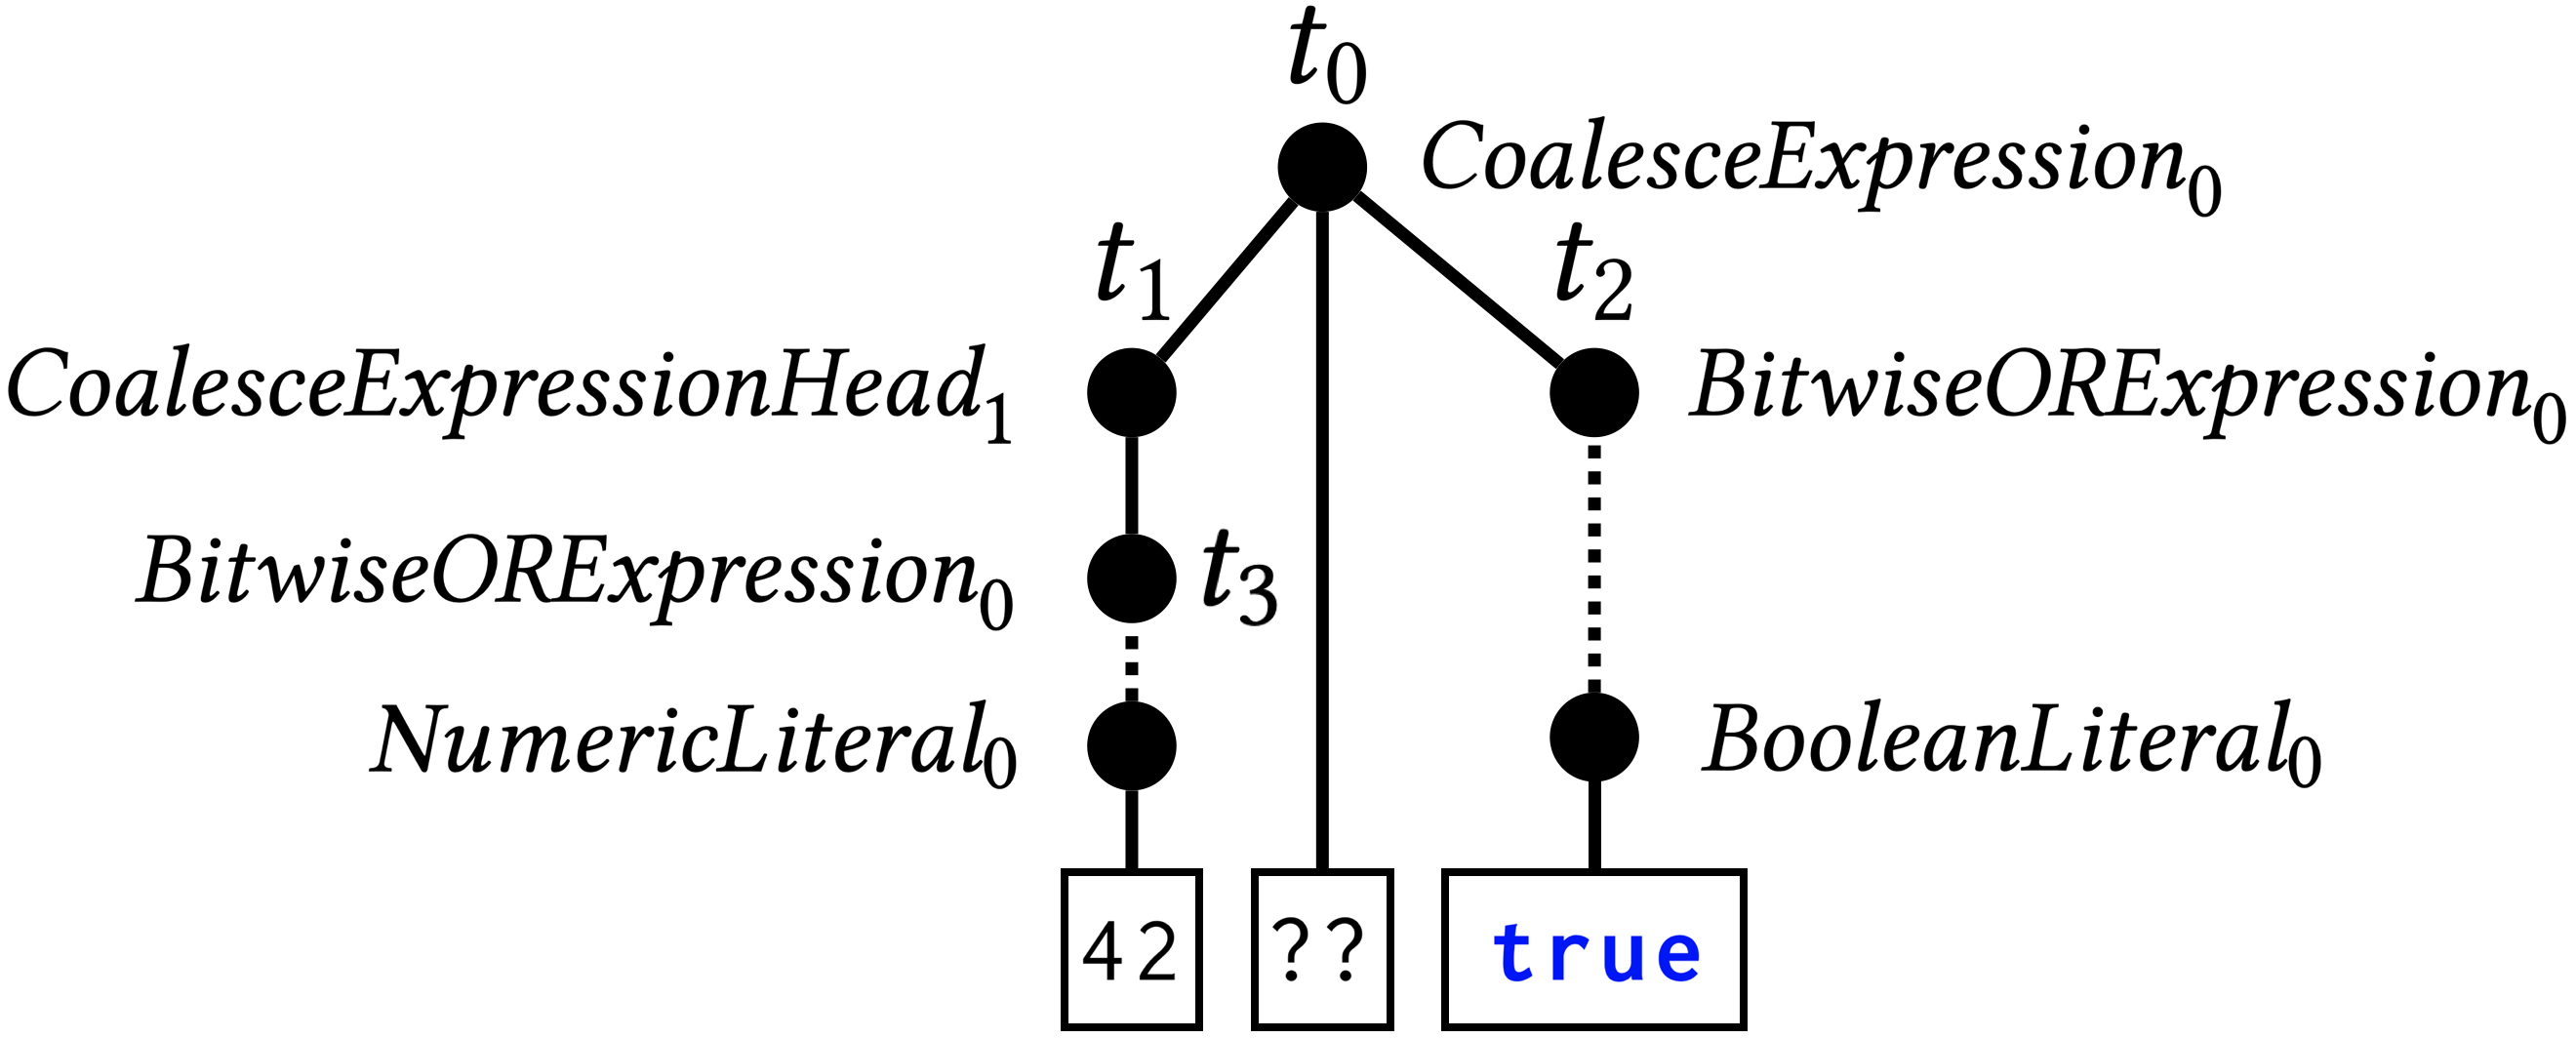
\includegraphics[width=.8\columnwidth]{img/ast-example.png}
\end{figure}
\noindent Its evaluation function $\nterm{CoalesceExpression}_0.\eval$ takes
three subtrees as arguments annotated by $\tree_0$, $\tree_1$, and $\tree_2$ in
the figure. Note that $\tree_1$ and $\tree_2$ are subtrees of $\tree_0$ (i.e.,
$\tree_1 \subtree \tree_0$ and $\tree_2 \subtree \tree_0$).


\begin{figure}
  \centering
  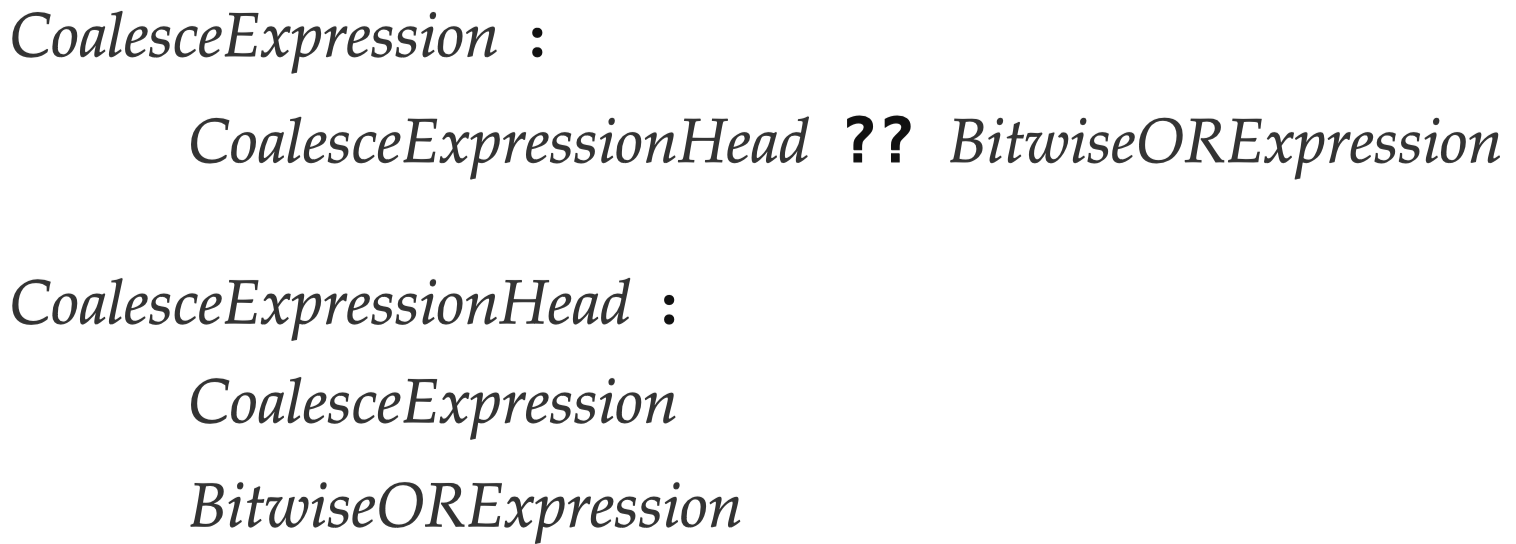
\includegraphics[width=.8\columnwidth]{img/coalesce-prod.png}
  \caption{A JavaScript syntactic production for coalesce expressions}
  \label{fig:coalesce-prod}
\end{figure}




\subsubsection{Concrete Semantics}

The concrete semantics $\sem{\prog}$ of an $\ires$ program $\prog = (\istset,
\getinst, \getnext)$ is defined as follows:
\[
  \sem{\prog} = \{ \st \in \stset \mid \ist \in \istset \wedge \ist \trans^* \st \}
\]
where $\trans^*$ denotes one or more repetition of $\trans$, and $\st \trans
\st'$ if and only if $\st = (\lab, \_, \_, \_)$ and $\sem{\getinst(\lab)}(\st) =
\st'$. Now, we define the denotational semantics of expressions, instructions,
and functions.

\paragraph{Expressions} We define the denotational semantics of expressions with
the following form:
\[
  \framebox{$\sem{\expr}: \stset \rightarrow \valset$}
\]
For each expression $\expr \in \exprset$, its semantics $\sem{\expr}$ takes a
state and returns a value as the result of expression. We define four different
cases in the semantics of expressions as
follows:
\begin{itemize}
  \item \underline{Primitive Values}:
    \[
      \sem{\pval}(\st) = \pval
    \]

  \item \underline{Operations}:
    \[
      \sem{\op \kwrl \expr_1, \cdots, \expr_n \kwrr}(\st) =
      \op(\val_1, \cdots, \val_n)
    \]
    where $\forall 1 \leq j \leq n. \; \sem{\expr_k}(\st) = \val_j$

  \item \underline{Variable Lookups}:
    \[
      \sem{\varx}(\st) = \env(\varx)
    \]
    where $\st = (\_, \_, \_, \env)$

  \item \underline{Field Lookups}:
    \[
      \sem{\expr_0 \kwsl \expr_1 \kwsr}(\st) = \val
    \]
    where
    \[
      \begin{array}{l@{~}c@{~}ll}
        \val_0 &=& \sem{\expr_0}(\st) &\wedge\\
        \val_1 &=& \sem{\expr_1}(\st) &\wedge\\
        \st &=& (\_, \_, \heap, \_) &\wedge\\
        \val &=& \left\{
          \begin{array}{ll}
            \heap(\addr)(\str)
            & \text{if} \; \val_0 = \addr \wedge \val_1 = \str\\

            \tree_j
            & \text{if} \; \val_0 = \ty_k \langle \tree_1, \cdots, \tree_n
            \rangle \wedge \val_1 = j\\
          \end{array}
        \right.\\
      \end{array}
    \]
\end{itemize}

\paragraph{Instructions} We define the denotational semantics of instructions
with the following form:
\[
  \framebox{$\sem{\inst}: \stset \rightarrow \stset$}
\]
For each instruction $\inst \in \instset$, its semantics $\sem{\inst}$ takes a
state and returns an updated state. We define six different cases in the
semantics of instructions as follows:

\begin{itemize}
  \item \underline{Variable Assignments}:
    \[
      \sem{\varx = \expr}(\st) =
      (\getnext(\lab), \ctxts, \heap, \env[\varx \mapsto \val])
    \]
    where $\sem{\expr}(\st) = ((\lab, \ctxts, \heap, \env), \val)$

  \item \underline{Field Assignments}:
    \[
      \sem{\expr_0 \kwsl \expr_1 \kwsr = \expr_2}(\st) =
      (\getnext(\lab), \ctxts, \heap[\addr \mapsto \obj'], \env)
    \]
    where
    \[
      \begin{array}{l@{~}c@{~}ll}
        \sem{\expr_0}(\st) &=& (\st', \addr) &\wedge\\
        \sem{\expr_1}(\st') &=& (\st'', \str) &\wedge\\
        \sem{\expr_2}(\st'') &=& ((\lab, \ctxts, \heap, \env), \val) &\wedge\\
        \obj &=& \heap(\addr) &\wedge\\
        \obj' &=& \obj[\str \mapsto \val]\\
      \end{array}
    \]

  \item \underline{Object Allocations}:
    \[
      \sem{\varx = \kwcl \kwcr}(\st) =
      (\lab, \ctxts, \heap[\addr \mapsto \epsilon], \env[\varx \mapsto
      \addr])
    \]
    where $\st = (\lab, \ctxts, \heap, \env) \wedge \addr \not\in
    \text{Domain}(\heap)$ and $\epsilon$ denotes an empty object.

  \item \underline{Function Calls}:
    \[
      \sem{\varx = \expr \kwrl \expr_1 \cdots \expr_n \kwrr}(\st) =
      (\lab_\varf, \ctxt :: \ctxts, \heap, \env')
    \]
    where
    \[
      \begin{array}{l@{~}c@{~}ll}
        \sem{\expr}(\st) &=& (\st_0, \kwdef \; \kwrl \varp_1, \cdots, \varp_n
        \kwrr \; \lab_\varf) &\wedge\\
        \sem{\expr_j}(\st_{j-1}) &=& (\st_j, \val_j) \;
        [\forall 1 \leq j \leq n] &\wedge\\
        \st_n &=& (\lab, \ctxts, \heap, \env) &\wedge\\
        \env' &=& [\varp_1 \mapsto \val_1, \cdots, \varp_n \mapsto \val_n]
        &\wedge\\
        \ctxt &=& (\getnext(\lab), \env, \varx)\\
      \end{array}
    \]

  \item \underline{Branches}:
    \[
      \sem{\kwif \; \expr \; \lab_\vart \; \lab_\varf}(\st) =
      \left\{
        \begin{array}{ll}
          (\lab_\vart, \ctxts, \heap, \env) & \text{if} \; \val = \true\\
          (\lab_\varf, \ctxts, \heap, \env) & \text{if} \; \val = \false\\
        \end{array}
      \right.
    \]
    where $\sem{\expr}(\st) = ((\lab, \ctxts, \heap, \env), \val)$

  \item \underline{Returns}:
    \[
      \sem{\kwret \; \expr}(\st) = (\lab, \ctxts, \heap, \env[\varx \mapsto
      \val])
    \]
    where $\sem{\expr}(\st) = ((\_, (\lab, \env, \varx) :: \ctxts, \heap, \_),
    \val)$
\end{itemize}


\subsection{Syntactic Views} A syntactic view $\atree \in \atreeset$ is an
augmented JavaScript ASTs with abstract nodes $\treetop$:
\[
  \atree ::= \term{\str} \mid \ty_k \langle \atree^* \rangle \mid \treetop
\]
and its concretization is defined as follows:
\[
  \begin{array}{lcl}
    \gamma(\term{\str}) &=&
    \{ \term{\str} \}\\

    \gamma(\ty_k \langle \atree_1, \cdots, \atree_n \rangle) &=&
    \{ \ty_k \langle \tree_1, \cdots, \tree_n \rangle \mid \tree_j \in
    \gamma(\atree_j) \}\\

    \gamma(\treetop) &=& \treeset\\
  \end{array}
\]
The partial order and join operator between abstract trees are defined as
follows:
\[
  \begin{array}{lcl}
    \atree \order \atree' &\Leftrightarrow& \left\{
      \begin{array}{ll}
        \atree = \atree' &\vee\\

        \atree' = \treetop &\vee\\

        \begin{array}{@{}l@{}}
          \atree = \ty_k \langle \atree_1, \cdots, \atree_n \rangle \wedge
          \atree' = \ty_k \langle \atree'_1, \cdots, \atree'_n \rangle \wedge\\
          \forall j. \; \tree_j \order \tree'_j\\
        \end{array}\\
      \end{array}
    \right.\\

    \atree \join \atree' &=& \left\{
      \begin{array}{ll}
        \atree' & \text{if} \; \atree \order \atree'\\

        \atree & \text{if} \; \atree \revorder \atree'\\

        \ty_k \langle \atree''_1, \cdots, \atree''_n \rangle &
        \text{if} \; \atree = \ty_k \langle \atree_1, \cdots, \atree_n \rangle
        \wedge\\&
        \phantom{\text{if} \;} \atree = \ty_k \langle \atree_1, \cdots, \atree_n
        \rangle \wedge\\&
        \phantom{\text{if} \;} \forall j. \; \atree''_j = \atree_j
        \join \atree'_j\\
        \treetop & \text{otherwise}\\
      \end{array}
    \right.\\
  \end{array}
\]
Moreover, we can filter out JavaScript programs using the subtree relation with
syntactic views:
\[
  \atree \subtree \tree' \iff \exists \tree \in \gamma(\atree). \; \tree
  \subtree \tree'
\]



\subsection{Partial Evaluation}

We define a \textit{partial evaluation} $\peval{-}: \progset \rightarrow
\atreeset \rightarrow \progset$ of $\ires$ programs to specialize JavaScript
semantics with a given syntactic view:
\[
  \peval{\prog}(\atree) = \transform(\prog, \asem{\prog}(\atree))
\]
It takes a syntactic view $\atree \in \atreeset$ to restrict arguments of the
corresponding evaluation function. Then, it performs a static analysis
$\asem{-}$ of a given program $\prog$ with the static part $\atree$ and
transforms it using $\transform$ with the analysis result
$\asem{\prog}(\atree)$ to produce a new specialized $\ires$ program.  Now, we
define the static analysis and program transformation of $\ires$ programs and
prove the semantics preservation of the partial evaluation consisting of them.

\subsubsection{Static Analysis}

To define static analysis of $\ires$ programs, we first define abstract domains
of states, calling contexts, environments, and values as follows:
\begin{itemize}
  \item \underline{Abstract States}:
    $\aelemset = \actxtset \times \afsenvset$
    \[
      \begin{array}{lcl}
        \gamma(\afsenv, \actxt) &=& \gamma(\actxt) \cap
        \gamma(\afsenv)\\

        (\actxt, \afsenv) \order (\actxt', \afsenv') &\Leftrightarrow&
        (\actxt \order \actxt') \wedge (\afsenv \order \afsenv')\\

        (\actxt, \afsenv) \join (\actxt', \afsenv') &=&
        (\actxt \join \actxt', \afsenv \join \afsenv')\\

        \bot &=& (\bot, \bot)\\

        \top &=& (\top, \top)\\
      \end{array}
    \]

  \item \underline{Abstract Calling Contexts}:
    $\actxtset = \funcset \finmap \powerset{\labset \times \varset}$
    \[
      \todo
      \begin{array}{lcl}
        \gamma(\actxt) &=& \{ \st \in \stset \mid
          \st = (\lab', (\lab, \_, \varx) :: \_, \_, \_) \wedge \\&&
          \phantom{\{ \st \in \stset \mid} (\lab, \varx) \in
            \actxt(\getfunc(\lab'))
        \}\\

        \actxt \order \actxt' &\Leftrightarrow&
        \forall \func \in \funcset. \; \actxt(\func) \subseteq \actxt'(\func)\\

        \actxt \join \actxt' &=&
        \lambda \func \in \funcset. \; \actxt(\func) \cup \actxt'(\func)\\

        \bot &=& \lambda \func \in \funcset. \; \bot\\

        \top &=& \lambda \func \in \funcset. \; \top\\
      \end{array}
    \]

  \item \underline{Flow-Sensitive Abstract Environments}:
    $\afsenvset = \labset \rightarrow \aenvset$
    \[
      \begin{array}{lcl}
        \gamma(\afsenv) &=& \{ \st \in \stset \mid
          \st = (\lab, \_, \_, \_) \wedge \st \in \gamma(\afsenv(\lab))
        \}\\

        \afsenv \order \afsenv' &\Leftrightarrow&
        \forall \lab \in \labset. \; \afsenv(\lab) \order \afsenv'(\lab)\\

        \afsenv \join \afsenv' &=&
        \lambda \lab \in \labset. \; \afsenv(\lab) \join \afsenv'(\lab)\\

        \bot &=& \lambda \lab \in \labset. \; \bot\\

        \top &=& \lambda \lab \in \labset. \; \top\\
      \end{array}
    \]

  \item \underline{Abstract Environments}:
    $\aenvset = \varset \rightarrow \aenvset$
    \[
      \begin{array}{lcl}
        \gamma(\aenv) &=& \{ \st \in \stset \mid
          \forall \varx \in \varset. \;
          \sem{\varx}(\st) \in \gamma(\aenv(\varx))
        \}\\

        \aenv \order \aenv' &\Leftrightarrow&
        \forall \varx \in \varset. \;
        \aenv(\varx) \order \aenv'(\varx)\\

        \aenv \join \aenv' &=&
        \lambda \varx \in \varset. \;
        \aenv(\varx) \join \aenv'(\varx)\\

        \bot &=& \lambda \varx \in \varset. \; \bot\\

        \top &=& \lambda \varx \in \varset. \; \top\\
      \end{array}
    \]

  \item \underline{Abstract Values}: $\avalset = \valset \uplus \atreeset \uplus
    \{ \bot, \top \}$
    \[
      \begin{array}{lcl}
        \gamma(\aval) &=& \left\{
          \begin{array}{ll}
            \{ \val \} & \text{if} \; \aval = \val\\
            \gamma(\atree) & \text{if} \; \aval = \atree\\
            \varnothing & \text{if} \; \aval = \bot\\
            \valset & \text{if} \; \aval = \top\\
          \end{array}
        \right.\\

        \aval \order \aval' &\Leftrightarrow& \left\{
          \begin{array}{ll}
            \aval = \bot \vee \aval' = \top \vee \aval = \aval' & \vee\\
            \aval = \atree \wedge \aval' = \atree' \wedge
            \atree \order \atree' &\vee\\
            \aval = \tree \wedge \aval' = \atree' \wedge \tree \in
            \gamma(\atree')\\
          \end{array}
        \right.\\

        \aval \join \aval' &=& \left\{
          \begin{array}{ll}
            \aval' & \text{if} \; \aval \order \aval'\\
            \aval & \text{if} \; \aval \revorder \aval'\\
            \top & \text{otherwise}\\
          \end{array}
        \right.\\
      \end{array}
    \]
\end{itemize}

An abstract state $\aelem \in \aelemset$ is a pair of an abstract calling
context and a flow-sensitive abstract environment.  An abstract calling context
$\actxt \in \actxtset$ is a mapping from functions to return labels and
variables in their calling contexts. A flow-sensitive abstract environment
$\afsenv \in \afsenvset$ is a mapping from labels to abstract environments to
represent the shape of environments in each label. An abstract environment
$\aenv \in \aenvset$ is a mapping from variables to abstract values to describe
values stored in variables. An abstract value $\aval \in \avalset$ is a static
value $\val$, a syntactic view $\atree$, a dynamic value $\top$, or nothing
$\bot$. Now, we define abstract semantics of expressions, instructions, and
programs.

\paragraph{Expressions} We first define abstract semantics of expressions as
follows:
\[
  \framebox{$\asem{\expr}: \aenvset \rightarrow \avalset$}
\]
\begin{itemize}
  \item \underline{Primitive Values}:
    \[
      \asem{\pval}(\aenv) = \pval
    \]
  \item \underline{Operations}:
    \[
      \asem{\op \kwrl \expr_1, \cdots, \expr_n \kwrr}(\aenv) = \aval
    \]
    where
    \[
      \begin{array}{l@{~}c@{~}l@{~}l}
        \asem{\expr_j}(\aenv) &=& \aval_j \; [\forall 1 \leq j \leq n]
        &\wedge\\
        \aval &=& \left\{
          \begin{array}{ll}
            \bot & \text{if} \; \exists j. \; \aval_j = \bot\\

            \op(\val_1, \cdots, \val_n) &
            \text{if} \; \forall j. \; \aval_j = \val_j\\

            \top & \text{otherwise}\\
          \end{array}
        \right.\\
      \end{array}
    \]
  \item \underline{Variable Lookups}:
    \[
      \asem{\varx}(\aenv) = \aenv(\varx)
    \]
  \item \underline{Field Lookups}:
    \[
      \asem{\expr_0 \kwsl \expr_1 \kwsr}(\aenv) = \aval
    \]
    where
    \[
      \begin{array}{l@{~}c@{~}l@{~}l}
        \asem{\expr_0}(\aenv) &=& \aval_0 &\wedge\\
        \asem{\expr_1}(\aenv) &=& \aval_1 &\wedge\\
        \aval &=& \left\{
          \begin{array}{ll}
            \tree_j & \text{if} \;
            \aval_0 = \ty_k \langle \tree_1, \cdots, \tree_n \rangle \wedge
            \aval_1 = j\\

            \atree_j & \text{if} \;
            \aval_0 = \ty_k \langle \atree_1, \cdots, \atree_n \rangle \wedge
            \aval_1 = j\\

            \top & \text{otherwise}\\
          \end{array}
        \right.\\
      \end{array}
    \]
\end{itemize}

\paragraph{Instructions} Then, we define the abstract semantics of instructions
using the abstract semantics of expressions as follows:
\[
  \todo
  \framebox{$\asem{\inst}: \labset \times \aenvset \rightarrow \aelemset
  \rightarrow \aelemset$}
\]
\begin{itemize}
  \item \underline{Variable Assignments}:
    \[
      \asem{\varx = \expr}(\lab, \aenv) =
      (\bot[\getnext(\lab) \mapsto \aenv[\varx \mapsto \aval]], \bot)
    \]
    where $\aval = \asem{\expr}(\aenv)$

  \item \underline{Field Assignments}:
    \[
      \asem{\expr_0 \kwsl \expr_1 \kwsr = \expr_2}(\lab, \aenv) =
      (\bot[\getnext(\lab) \mapsto \aenv], \bot)
    \]
  \item \underline{Object Allocations}:
    \[
      \asem{\varx = \kwcl \kwcr}(\lab, \aenv) =
      (\bot[\getnext(\lab) \mapsto \aenv[\varx \mapsto \top]], \bot)
    \]

  \item \underline{Function Calls}:
    \[
      \asem{\varx = \expr \kwrl \expr_1 \cdots \expr_n \kwrr}(\lab, \aenv) =
      \text{\todo extensible target functions}
    \]
    where
    \[
      \begin{array}{l@{~}c@{~}ll}
        \aval' = \asem{\expr}(\aenv) &\wedge\\
        (\expr'_j, \_) = \transforme(\expr_j, \aenv) \; [\forall 1 \leq j \leq
        n]\\
      \end{array}
    \]

  \item \underline{Branches}:
    \[
      \asem{\kwif \; \expr \; \lab_\vart \; \lab_\varf, \aenv} =
      (\kwif \; \expr' \; \lab_\vart \; \lab_\varf, \aenv)
    \]
    where
    \[
      (\expr', \_) = \transforme(\expr, \aenv)
    \]

  \item \underline{Returns}:
    \[
      \asem{\kwret \; \expr, \aenv} =
      (\kwret \; \expr, \aenv)
    \]
    where
    \[
      (\expr', \_) = \transforme(\expr', \aenv)
    \]
\end{itemize}

% \paragraph{Transformation of Programs} Finally, we define the transformation
% of programs as the least fixed point of the abstract transfer function:
% \[
%   \transform(\prog, (\func, (\aval_1, \cdots, \aval_n))) = \lfp \; \atransfer =
%   \lim_{n \rightarrow \infty}(\atransfer)^n(\prog, \iaelem)
% \]
% where
% \begin{itemize}
%   \item \underline{Abstract Transfer Function}: $\atransfer: \progset \times
%     \aelemset \rightarrow \progset \times \aelemset$
%     \[
%       \atransfer(\prog, \aelem) = \lambda \lab \in \labset. \; \bigjoin_{\lab' \in
%       \labset}{\todo}
%     \]
%     where
%     \[
%     \]
%   \item \underline{Initial Abstract State}: $\iaelem \in \elemset$
%     \[
%       \iaelem = \todo
%     \]
% \end{itemize}
% 
% \todo

\subsubsection{Transformations}

\todo

% \[
%   \framebox{$\transforme: \exprset \times \aenvset \rightarrow \exprset \times
%   \avalset$}
% \]
% \[
%   \transforme(\expr, \aenv) = (\expr'', \aval)
% \]
% where
% \[
%   \begin{array}{l@{~}c@{~}ll}
%     \aval &=& \asem{\expr}(\aenv) &\wedge\\
%     \expr'' &=& \left\{
%       \begin{array}{ll}
%         \pval & \text{if} \; \aval = \langle \pval, \_ \rangle\\
%         \expr' & \text{if} \; \aval = \langle \_, \expr' \rangle\\
%         \expr & \text{otherwise}\\
%       \end{array}
%     \right.\\
%   \end{array}
% \]

% \[
%   \framebox{$\transformi: \instset \times \aenvset \rightarrow \instset \times
%   \aenvset$}
% \]
% \begin{itemize}
%   \item \underline{Variable Assignments}:
%     \[
%       \transformi(\varx = \expr, \aenv) =
%       (\varx = \expr', \aenv[\varx \mapsto \aval])
%     \]
%     where
%     \[
%       (\expr', \aval) = \transforme(\expr, \aenv)
%     \]
% 
%   \item \underline{Field Assignments}:
%     \[
%       \transformi(\expr_0 \kwsl \expr_1 \kwsr = \expr_2, \aenv) =
%       (\expr'_0 \kwsl \expr'_1 \kwsr = \expr'_2, \aenv)
%     \]
%     where
%     \[
%       \begin{array}{l@{~}c@{~}ll}
%         (\expr'_0, \_) = \transforme(\expr_0, \aenv) &\wedge\\
%         (\expr'_1, \_) = \transforme(\expr_1, \aenv) &\wedge\\
%         (\expr'_2, \_) = \transforme(\expr_2, \aenv)\\
%       \end{array}
%     \]
%   \item \underline{Object Allocations}:
%     \[
%       \transformi(\varx = \kwcl \kwcr, \aenv) =
%       (\varx = \kwcl \kwcr, \aenv[\varx \mapsto \top])
%     \]
% 
%   \item \underline{Function Calls}:
%     \[
%       \transformi(\varx = \expr \kwrl \expr_1 \cdots \expr_n \kwrr, \aenv) =
%       (\varx = \expr' \kwrl \expr'_1 \cdots \expr'_n \kwrr,
%       \aenv[\varx \mapsto \top])
%     \]
%     where
%     \[
%       \begin{array}{l@{~}c@{~}ll}
%         (\expr', \_) = \transforme(\expr, \aenv) &\wedge\\
%         (\expr'_k, \_) = \transforme(\expr_k, \aenv) \; \forall 1 \leq k \leq
%         n\\
%       \end{array}
%     \]
% 
%   \item \underline{Branches}:
%     \[
%       \transformi(\kwif \; \expr \; \lab_\vart \; \lab_\varf, \aenv) =
%       (\kwif \; \expr' \; \lab_\vart \; \lab_\varf, \aenv)
%     \]
%     where
%     \[
%       (\expr', \_) = \transforme(\expr, \aenv)
%     \]
% 
%   \item \underline{Returns}:
%     \[
%       \transformi(\kwret \; \expr, \aenv) =
%       (\kwret \; \expr, \aenv)
%     \]
%     where
%     \[
%       (\expr', \_) = \transforme(\expr', \aenv)
%     \]
% \end{itemize}



\subsubsection{Cleanup Algorithm}

\todo

\begin{itemize}
  \item perform a syntactic def-use analysis
  \item remove unnecessary variable assignments
  \item remove unreachable instructions
\end{itemize}


\subsubsection{Proof of Semantics Preservation}

\todo





\subsection{JavaScript Semantics Specialization}

This section explains how to utilize the partial evaluation for the JavaScript
semantics specialization with a user-defined syntactic view.  We first formally
define syntactic views and their operations, then we explain how to decide a
restriction of the constant propagation specialization based on a given
syntactic view.

\subsubsection{Semantics Specialization}

\todo
